% VUT FIT 1MITAI
% TIN 2019/2020
% Project: Task 2
% Author: Vladimir Dusek, xdusek27
% Date: 2/12/2019
% File: xdusek27.tex

%%%%%%%%%%%%%%%%%%%%%%%%%%%%%%%%%%%%%%%%%%%%%%%%%%%%%%%%%%%%%%%%%%%%%

\documentclass[11pt, a4paper, titlepage]{article}
\usepackage[left=2cm, text={17cm, 24cm}, top=3cm]{geometry}
\usepackage[utf8]{inputenc}
\usepackage[czech]{babel}
\usepackage{pdfpages}
\usepackage{amssymb}
\usepackage{multicol}
\usepackage{enumitem}
\usepackage{amsmath}
\usepackage{scrextend}

\newcommand{\N}{\mathbb{N}_0}

\setlength\parindent{0pt}

%%%%%%%%%%%%%%%%%%%%%%%%%%%%%%%%%%%%%%%%%%%%%%%%%%%%%%%%%%%%%%%%%%%%%

\begin{document}

\begin{titlepage}
    \begin{center}
        \begin{figure}[htb]
            \centering
            
\includegraphics[width=0.85\hsize]{images/fitlogo.pdf}
        \end{figure}
        \vspace{\stretch{0.382}}
        {\Huge Teoretická informatika} \\
        \bigskip
        {\LARGE Úkol 2} \\
        \vspace{\stretch{0.618}}
    \end{center}
    {\Large \today \hfill Vladimír Dušek, xdusek27}
\end{titlepage}

%%%%%%%%%%%%%%%%%%%%%%%%%%%%%%%%%%%%%%%%%%%%%%%%%%%%%%%%%%%%%%%%%%%%%

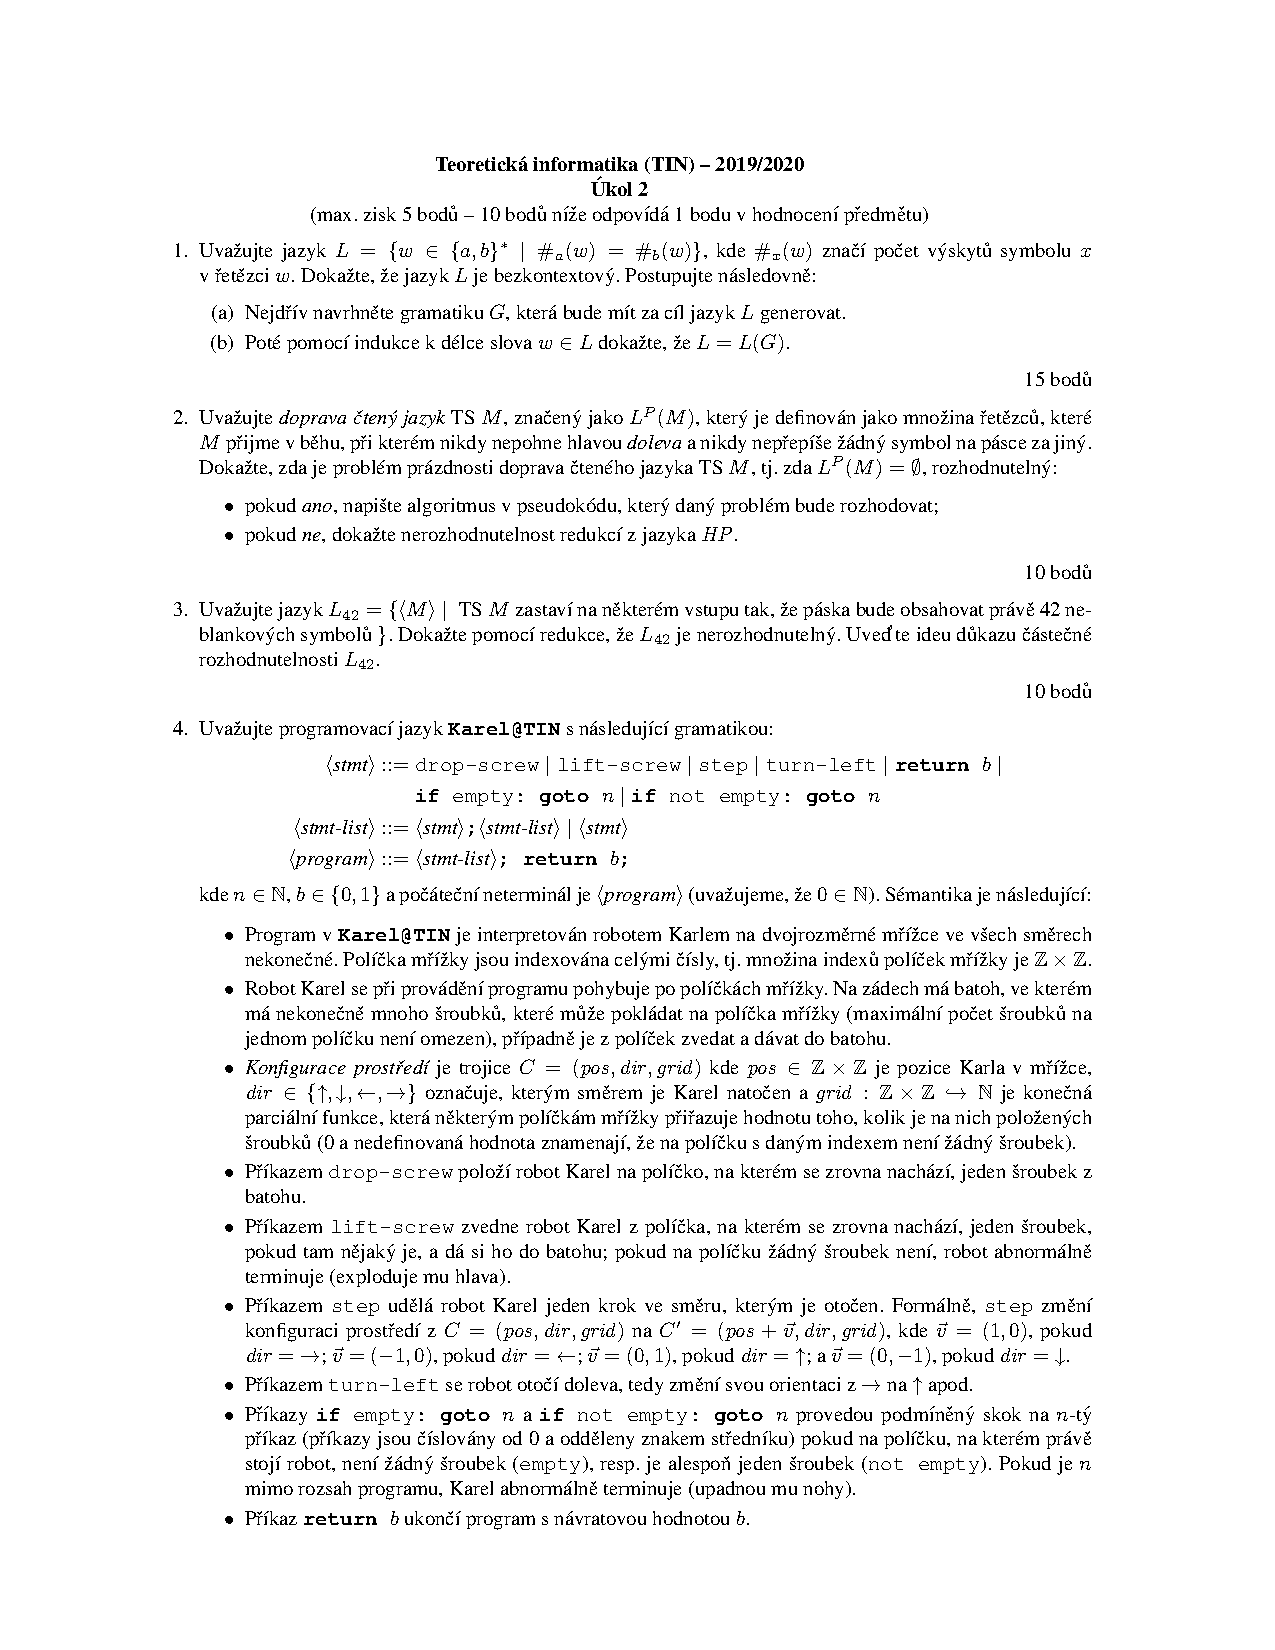
\includepdf[pages=1]{assignment.pdf}
\includepdf[pages=2]{assignment.pdf}

%%%%%%%%%%%%%%%%%%%%%%%%%%%%%%%%%%%%%%%%%%%%%%%%%%%%%%%%%%%%%%%%%%%%%

\section*{Příklad 1}

Máme jazyk $L = \{ w \in \{ a, b \}^* \mid \#_a(w) = \#_b(w) \}$. Navrhněme gramatiku $G$, která jazyk $L$ generuje:

$$
    G = (
        \{S\},
        \{a, b\},
        \{S \rightarrow \varepsilon \mid SaSb \mid aSbS \mid SbSa \mid bSaS\},
        S
    )
$$

Nyní indukcí k délce slova dokažme, že gramatika $G$ skutečně generuje jazyk $L$. Tedy, že $L = L(G)$. Postupně ukážeme, že $L(G) \subseteq L$ a $L \subseteq L(G)$, z toho poté přímo vyplývá, že $L = L(G)$. Nechť $i$ je délka slova.
\bigskip
\bigskip



\textbf{Tvrzení 1:} jestliže řetězec $w$ je generován gramatikou $G$, pak $w \in L$. Tedy, že $L(G) \subseteq L$.
\bigskip

\textit{Základní případy:}

\begin{itemize}
    \item $i = 0$. Jediný řetězec délky $0$ je $\varepsilon$ (prázdný řetězec). Jelikož derivace $S \Rightarrow \varepsilon$ je součástí gramatiky $G$, tak $\varepsilon \in L(G)$. Zároveň $\varepsilon$ obsahuje stejný počet symbolů $a$ a $b$ ($0$), proto $\varepsilon \in L$. Z toho vyplývá, že pro $i = 0$ tvrzení $L(G) \subseteq L$ platí.

    \item $i = 2$. Možné řetězce délky $2$ nad $\{ a, b \}^*$ jsou $aa, ab, ba, bb$. Jelikož derivace $S \Rightarrow SaSb \Rightarrow aSb \Rightarrow ab$ a $S \Rightarrow SbSa \Rightarrow bSa \Rightarrow ba$ jsou součástí gramatiky $G$, tak $ab, ba \in L(G)$. Obdobné derivace, které by generovaly řetězce $aa, bb$ nejsou součástí gramatiky $G$, proto $aa, bb \notin L(G)$. Zároveň řetězce $ab, ba$ obsahují stejný počet symbolů $a$ a $b$ ($1$), proto $ab, ba \in L$. Řetězce $aa, bb$ neobsahují stejný počet symbolů $a$ a $b$, proto $aa, bb \notin L$. Z toho vyplývá, že pro $i = 2$ tvrzení $L(G) \subseteq L$ platí.
\end{itemize}

\medskip
\textit{Indukční hypotéza:}

\begin{itemize}
    \item Předpokládejme, že pro všechny řetězce $w$ takové, že $|w| \leq i$, platí $w \in L(G) \Rightarrow w \in L$.
\end{itemize}

\medskip
\textit{Indukční krok:}

\begin{itemize}
    \item Ukažme platnost tvrzení pro délku slova $i+2$. Je zřejmé, že řetězce délky $i+1$ nejsou součástí jazyka $L(G)$, jelikož všechna pravidla generují sudý počet terminálních symbolů.

    \item Uvažujme řetězec $w_j \in L(G)$ délky $i+2$. Mohou nastat následující situace:
\end{itemize}

\begin{itemize}[leftmargin=2cm, label=$\circ$]
    \item $S \Rightarrow aSbS \Rightarrow^* a u_1 b v_1 = w_1$, kde $|u_1| + |v_1| = i$
    \item $S \Rightarrow SaSb \Rightarrow^* u_2 a v_2 b  = w_2$, kde $|u_2| + |v_2| = i$
    \item $S \Rightarrow bSaS \Rightarrow^* b u_3 a v_3 = w_3$, kde $|u_3| + |v_3| = i$
    \item $S \Rightarrow SbSa \Rightarrow^* u_4 b v_4 a = w_4$, kde $|u_4| + |v_4| = i$
\end{itemize}

\begin{itemize}
    \item Na základě indukční hypotézy, kdy předpokládáme, že z počátečního neterminálu $S$ dokážeme po konečném počtu kroků vygenerovat slovo délky maximálně $i$, můžeme uvážit podmínky $|u_j| + |v_j| = i$ pro $j \in \{1, 2, 3, 4\}$.

    \item Jelikož $u_j, v_j \in L(G)$, tak dle indukční hypotézy $u_j, v_j \in L$.

    \item Tvrzení $L(G) \subseteq L$ platí i pro $i + 2$.
\end{itemize}
\newpage



\textbf{Tvrzení 2:} jestliže řetězec $w \in L$, pak $w$ je generován gramatikou $G$. Tedy, že $L \subseteq L(G)$.
\bigskip

\textit{Základní případy:}

\begin{itemize}
    \item $i = 0$. Jediný řetězec délky $0$ je $\varepsilon$ (prázdný řetězec). Řetězec $\varepsilon$ obsahuje stejný počet symbolů $a$ a $b$ ($0$), proto $\varepsilon \in L$. Zároveň derivace $S \Rightarrow \varepsilon$ je součástí gramatiky $G$, tedy $\varepsilon \in L(G)$. Z toho vyplývá, že pro $i = 0$ tvrzení $L \subseteq L(G)$ platí.

    \item $i = 2$. Možné řetězce délky $2$ nad $\{ a, b \}^*$ jsou $aa, ab, ba, bb$. Řetězce $ab, ba$ obsahují stejný počet symbolů $a$ a $b$ ($1$), proto $ab, ba \in L$. Řetězce $aa, bb$ neobsahují stejný počet symbolů $a$ a $b$, proto $aa, bb \notin L$. Jelikož derivace $S \Rightarrow SaSb \Rightarrow aSb \Rightarrow ab$ a $S \Rightarrow SbSa \Rightarrow bSa \Rightarrow ba$ jsou součástí gramatiky $G$, tak $ab, ba \in L(G)$. Obdobné derivace, které by generovaly řetězce $aa, bb$ nejsou součástí gramatiky $G$, proto $aa, bb \notin L(G)$. Z toho vyplývá, že pro $i = 2$ tvrzení $L \subseteq L(G)$ platí.
\end{itemize}

\medskip
\textit{Indukční hypotéza:}

\begin{itemize}
    \item Předpokládejme, že pro všechny řetězce $w$ takové, že $|w| \leq i$, platí $w \in L \Rightarrow w \in L(G)$.
\end{itemize}

\medskip
\textit{Indukční krok:}

\begin{itemize}
    \item Ukažme platnost tvrzení pro délku slova $i+2$. Je zřejmé, že řetězce délky $i+1$ nejsou součástí jazyka $L$, jelikož nemohou obsahovat stejný počet symbolů $a$ a $b$.

    \item Uvažujme řetězec $w_j \in L$ délky $i+2$. Mohou nastat následující situace:
\end{itemize}

\begin{itemize}[leftmargin=2cm, label=$\circ$]
    \item $w_1 = a v_1 b$, kde $v_1 \in L$
    \item $w_2 = b v_2 a$, kde $v_2 \in L$
    \item $w_3 = a v_3 a$, kde $v_3 \in \{ w \mid w \in \{ a, b \}^* \land \#_a(w) - 2 = \#_b(w) \}$
    \item $w_4 = b v_4 b$, kde $v_4 \in \{ w \mid w \in \{ a, b \}^* \land \#_a(w) = \#_b(w) - 2 \}$
\end{itemize}

\begin{itemize}
    \item V gramatice $G$ pak existují derivace:
\end{itemize}

\begin{itemize}[leftmargin=2cm, label=$\circ$]
    \item $S \Rightarrow aSbS \Rightarrow aSb \Rightarrow^* w_1$
    \item $S \Rightarrow bSaS \Rightarrow bSa \Rightarrow^* w_2$
    \item $S \Rightarrow aSbS \Rightarrow aSbSbSa \Rightarrow^* w_3$
    \item $S \Rightarrow bSaS \Rightarrow bSaSaSb \Rightarrow^* w_4$
\end{itemize}

\begin{itemize}
    \item Tvrzení $L \subseteq L(G)$ platí i pro $i + 2$.
\end{itemize}
\bigskip



\textbf{Závěr:} bylo dokázáno tvrzení 1 i tvrzení 2, z toho vyplývá že $L = L(G)$.


% https://www.eecs.yorku.ca/course_archive/2006-07/F/2001/handouts/lect11-supplement.pdf

% https://cs.stackexchange.com/questions/18524/how-to-prove-that-a-language-is-context-free

% https://cs.stackexchange.com/questions/11315/how-to-show-that-l-lg

% https://github.com/Romop5/FITVUT-TIN-2018-Homeworks/tree/master/2

\newpage

%%%%%%%%%%%%%%%%%%%%%%%%%%%%%%%%%%%%%%%%%%%%%%%%%%%%%%%%%%%%%%%%%%%%%

\section*{Příklad 2}

Problém $L^P(M) = \emptyset$ je rozhodnutelný a řeší ho například následující algoritmus.
\bigskip

\textbf{Návrh algoritmu}

\begin{itemize}

    \item \textbf{Vstup:} Turingův stroj $M = (Q, \Sigma, \Gamma, \delta, q_0, g_f)$
    \item \textbf{Výstup:} $L^P(M) = \emptyset$ nebo $L^P(M) \neq \emptyset$
    \item \textbf{Metoda:} \begin{enumerate}

        \item Postupně transformujeme turingův stroj $M$ na rozšířený konečný automat $M'$.
        $$M' = (Q', \Sigma, \delta', q_0, F)$$

        \item Množina stavů $Q' \subseteq Q$:
        $$Q' = \{q_0\} \cup \{q \mid q \in Q \land \exists a \in \Sigma \cup \{\Delta\} \; \exists p \in Q : (p, a) \rightarrow (q, R) \in \delta \}$$

        % \{q \mid q \in Q \land \exists a \in \Sigma \cup \{\Delta\} \; \exists p \in Q : (p, a) \rightarrow (q, R) \in \delta \}$$

        \item Přechodová funkce $\delta'$:\footnote{Je vhodné doplnit, že symbol $\Delta$ značící prázdný symbol v přechodové funkci $\delta$ je ekvivalentní se symbolem $\varepsilon$, značící prázdný řetězec v přechodové funkci $\delta'$.}
        $$\delta' = \{ (q, a) \rightarrow p \mid q, p \in Q' \land a \in \Sigma \cup \{\Delta\} \land (q, a) \rightarrow (p, R) \in \delta \} \, \cup$$
        $$\cup \, \{ (q, a) \rightarrow p \mid q, p \in Q' \land a \in \Sigma \cup \{\Delta\} \land \exists q_1, ..., q_n \in Q : $$
        $$ : (q, a) \rightarrow (q_1, a) \in \delta \land (q_1, a) \rightarrow (q_2, a) \in \delta \land ... \land (q_n, a) \rightarrow (p, R) \in \delta\}$$

        \item Množina koncových stavů $F$:
        $$F = \{q_f\}$$

        \item Rozšířený konečný automat $M'$ převedeme dle algoritmu 3.6\footnote{http://www.fit.vutbr.cz/study/courses/TIN/public/Texty/TIN-studijni-text.pdf} na deterministický konečný automat $M''$.
        $$M'' = (Q'', \Sigma, \delta'', q_0', F)$$

        \item Jazyk $L(M'') = L^P(M) \in \mathcal{L}_3$ a dle věty 3.2$^2$ je problém neprázdnosti jazyka ve třídě $\mathcal{L}_3$ rozhodnutelný. A sice:
        $$\exists w \in \Sigma^* : (q_0', w) \vdash^* (q_f, \varepsilon) \Rightarrow L^P(M) \neq \emptyset$$
        $$\nexists w \in \Sigma^* : (q_0', w) \vdash^* (q_f, \varepsilon) \Rightarrow L^P(M) = \emptyset$$

    \end{enumerate}

\end{itemize}

\newpage

%%%%%%%%%%%%%%%%%%%%%%%%%%%%%%%%%%%%%%%%%%%%%%%%%%%%%%%%%%%%%%%%%%%%%

\section*{Příklad 3}

Nerozhodnutelnost problému $L_{42}$ dokážeme zavedním redukce $\sigma$ z problému nezastavení ($L_{CoHP}$). Nejprve si uvedené jazyky formálně definujeme.

\begin{itemize}

    \item $L_{42} = \{ \langle M \rangle \mid \textrm{TS} \, M \, \textrm{definovaný kódem} \, \langle M \rangle \, \textrm{zastaví na některém vstupu tak, že páska bude}$

    $\textrm{obsahovat právě} \, 42 \, \textrm{neblankových symbolů} \, \} \subseteq \{0, 1\}^*$

    \item $L_{CoHP} = \{ \langle M \rangle \# \langle w \rangle \mid \textrm{TS} \, M \, \textrm{definovaný kódem} \, \langle M \rangle \, \textrm{na vstupu} \, w \, \textrm{definovaným kódem} \, \langle w \rangle$

    $\textrm{nezastaví} \, \} \subseteq \{0, 1, \#\}^*$

\end{itemize}
\medskip

\textbf{Myšlenka redukce}
\bigskip

Funkce $\sigma$ je realizována úplným turingovým strojem $M_{\sigma}$ tak, že pro instanci $x \in L_{CoHP}$  zapíše na výstupní pásku kód turingova stroje $M_x$, který se chová následovně:

\begin{enumerate}

\item Vymaže obsah svoji vstupní pásky.

\item Na vstupní pásku zapíše řetězec $x=x_1 \# x_2$, ze kterého byl sám vygenerován. Ten má uložen jako konstantu ve svém stavovém řízení.

\item Provede analýzu, zda řetězec $x$ je platnou instancí $L_{CoHP}$. Pokud ne, odmítne, a tedy $L(M_x) = \emptyset$.

\item Odsymuluje běh turingova stroje s kódem $x_1$ na vstupu s kódem $x_2$ s využitím univerzálního turingova stroje, který je jeho komponentou. Pokud běh skončí, pak pokračuje dalším krokem, jinak cyklí.

\item Po dokončení běhu spočítá počet neblankových symbolů na pásce. Pokud napočítá $43$, tak přijme a $L(M_x) = \{0, 1\}^*$. Pokud je na pásce méně než $43$ neblankových symbolů bude cyklit.

\end{enumerate}
\medskip

\textbf{Realizace redukce}
\bigskip

\begin{itemize}

\item $M_\sigma$ lze realizovat jako úplný turingův stroj. $M_\sigma$ vygeneruje kód turingova stroje $M_x$, který se skládá z několika menších komponent mezi kterými předává řízení. Jedná se o komponenty:

\begin{enumerate}

\item Kód turingova stroje $M_{erase}$ pro smazání vstupní pásky. Všechny výchozí symboly na pásce, přepíše na $\Delta$.

\item Kód turingova stroje $M_{write\,\_\,x}$, který na vstupní pásku zapíše řetězec $x$. Posouvá hlavu doprava a zapisuje jednotlivé symboly řetězce $x$.

\item Kód turingova stroje $M_{valid}$, který ověří, jestli řetězec $x = x_1 \# x_2$ je platnou instancí $L_{CoHP}$. Jedná se o test na členství v regulárním jazyce.

\item Kód univerzálního turingova stroje $M_{UTS}$ pro simulaci chování turingova stroje na daném vstupu.

\item Kód turingova stroje $M_{more\,\_\,42}$ pro počítání neblankových symbolů. Ten má $44$ řídících stavů a v každém z nich, kromě posledního koncového, buď přes $\Delta$ cyklí a posunuje čtecí hlavou doprava, nebo přes cokoliv jiného přechází do dalšího stavu a čtecí hlavou posunuje taktéž doprava. V momentě, kdy dojde do koncového stavu, je na pásce 43, nebo více symbolů.

\item Pomocnou logiku pro propojení výstupů s vstupy jednotlivých komponent.

\end{enumerate}

\item Redukce je potom funkce $\sigma : \{0, 1, \#\}^* \rightarrow \{0, 1\}^*$, která je realizována úplným turingovým strojem $M_\sigma$.

\end{itemize}

% \newpage

%%%%%%%%%%%%%%%%%%%%%%%%%%%%%%%%%%%%%%%%%%%%%%%%%%%%%%%%%%%%%%%%%%%%%

% \section*{Příklad 4}

% ToDo

% \newpage

%%%%%%%%%%%%%%%%%%%%%%%%%%%%%%%%%%%%%%%%%%%%%%%%%%%%%%%%%%%%%%%%%%%%%

\end{document}
